\section{Optimization Algorithms}

For most control problems involving dynamic equations and contacts,
the objective function $\hat{f}(\boldsymbol{\phi})$ (\eqnref{optskills_disccost})
is highly non-convex and often non-differentiable.
A common practice is to use a sampling-based
optimization algorithm to find the optimal solution. In particular,
CMA-ES \cite{Hansen:2003:CMA} has been successfully applied to many
  high-dimensional control problems. We will first summarize the core ideas
  of CMA-ES and use it as a baseline to compare with our new optimization algorithm.

\subsection{Baseline algorithm: CMA-ES}
CMA-ES is a sampling-based, derivative-free evolutionary
algorithm for solving optimization problems. The evolution process
updates a multivariate normal distribution 
\begin{equation}
  \begin{aligned}
    \vc{x}_k \mytilde \vc{m} + \sigma \mathcal{N}(\vc{0},
    \mat{C}) \text{ for } k = 1 .. \lambda
  \end{aligned}
\end{equation} 
where $\vc{m}$ is the mean, $\sigma$ is the step size, and
$\mathcal{N}(\vc{0}, \mat{C})$ is the multivariate normal distribution
with zero mean and covariance matrix $\mat{C}$. Initially, $\vc{m}$ is
set to zero and $\mat{C}$ is set to identity. In each generation,
$\lambda$ new candidates are sampled from the current multivariate
normal distribution. All the samples are evaluated by the objective
function and the best $\mu$ samples are selected to update the mean
and the covariance matrix for the next generation. When the
termination criteria are met, the final mean value is output as the
optimal point of the optimization.  A number of follow-on research
introduced different schemes for sample selection and different rules
for updating the probability distribution. A comprehensive
introduction can be found in the tutorial by Hansen \etal \cite{Hansen:2003:CMA}.

% \updated{\st{One common strategy is to create a pool of samples that
%     consists of $\lambda$ new samples and $\mu$ old samples from the previous generation,
%     and select the best $\mu$ samples from this pool.}
%   One common strategy is selecting the best $\mu$ samples from $\lambda$ new
%   samples while discarding all previous elite samples.}
% These new samples are used to update the mean and the covariance
% matrix for the next generation. When the termination criteria are met,
% the mean value is output as the optimal point of the optimization.

The rule for adapting covariance matrix is a key characteristic of
CMA-ES.  Among different versions, (1+1)-CMA-ES \cite{Igel:2006:CEG}
has the simplest mechanism to evolve covariance matrix. In every
generation, if a sample is not better than the mean from the previous
generation, it will be discarded and a new one will be drawn. The
process repeats until a better sample is generated (called elite
sample). The elite sample will replace the mean and update the
covariance matrix via a procedure called \textbf{updateCov}, which
details are summarized in Appendix. \textbf{updateCov} takes as
input the previous mean and the elite sample, and outputs the adapted
covariance matrix $\mat{C}$. 
 
%  the
% procedure \emph{updateCov}.  When a new sample $\vc{x}$ is better than
% the previous mean $\vc{x}'$, \emph{updateCov} takes a difference
% vector $\vc{y}=\vc{x}-\vc{x}'$ and gradually learns the covariance
% matrix $\mat{C}$.  In the later section, we will update our covariance
% matrices using this routine.  Please refer the appendix for
% mathematical details.

\subsection{Our Algorithm for Parameterized Optimization Problem}
\label{sec:optskills_our_algorithm}

Directly applying CMA-ES to solve a parameterized optimization problem
is difficult due to the expanded dimensionality. Consider a policy
parameter space $\mathcal{X} = \mathcal{R}^n$ and a cubic
representation for the parameterized skill function,
$\vc{x}_{\boldsymbol{\phi}}(w)$, where $\mathcal{F} =
\mathcal{R}^{4n}$. The dimension of $\mathcal{F}$ can be higher if we
use more complex function forms to represent
$\vc{x}_{\boldsymbol{\phi}}(w)$. Sampling in the high-dimensional
$\mathcal{F}$ can result in very slow convergence for CMA-ES.

We propose a new sampling-based algorithm to combat the issue of
expanded dimensionality. Our key idea is to sample in the space of
policy parameters, $\mathcal{X}$, instead of the space of
$\mathcal{F}$. This alternative sampling space will lead to the same solution
because there is a one-to-one mapping between a point in $\mathcal{F}$
and a curve segment in $\mathcal{X}$. Using CMA-ES to evolve the
mean point in $\mathcal{F}$ is equivalent to evolving the \emph{mean
  segment} in $\mathcal{X}$.  The obvious advantage of drawing
samples from the space of policy parameters is that the dimensionality
is invariant to the complexity of the parameterized skill
function. Moreover, evaluating a sample $\vc{x}$ only requires one
trial of a simulation $\mathcal{S}(\vc{x})$ (\eqnref{optskills_paramcost}), while evaluating a sample $\boldsymbol{\phi}$ requires
integration of $f$ over $w \in [0,1]$.  Using the discretized
approximation shown in \eqnref{optskills_disccost}, every evaluation of
$\boldsymbol{\phi}$ costs $M$ simulation trials.
 
Since we are solving for a solution segment rather than a single
solution point, 
the definitions of the mean and covariance matrix also need to be
modified. We define a continuous function: $\vc{m}_{\boldsymbol{\phi}}(w)$
$: [0, 1] \mapsto \mathcal{R}^n$ to represent the \emph{mean
  segment}. Similarly, we also need to parameterize the covariance matrix
$\mat{C}$ with the task interpolation parameter as
$\mat{C}(w)$.
%% \karen{We need to explain that $\mat{C}(w)$ is not
%%   continuously defined alone w, unlike
%%   $\vc{m}_{\boldsymbol{\phi}}(w)$. Instead, $\mat{C}(w)$ is just $M$
%%   discrete covariance matrices. We will need this
%%   information for drawing samples followed immediately.}
Unlike the \emph{mean segment}, we do not represent $\mat{C}(w)$ as
a continuous function because accurate estimation of
continuous $\mat{C}(w)$ requires a large number of sample evaluations. We
choose a simpler way to estimate the covariance of the 
parameterized probability function by maintaining one covariance matrix $\mat{C}(w_i)$
for each discretized task interpolation parameter $w_i$.
%% \karen{unnecessary info at this point.}
%%  \updated{and applying
%%   \textbf{updateCov} routine that requires only one sample per covariance.}

\begin{figure}[t]
\center
  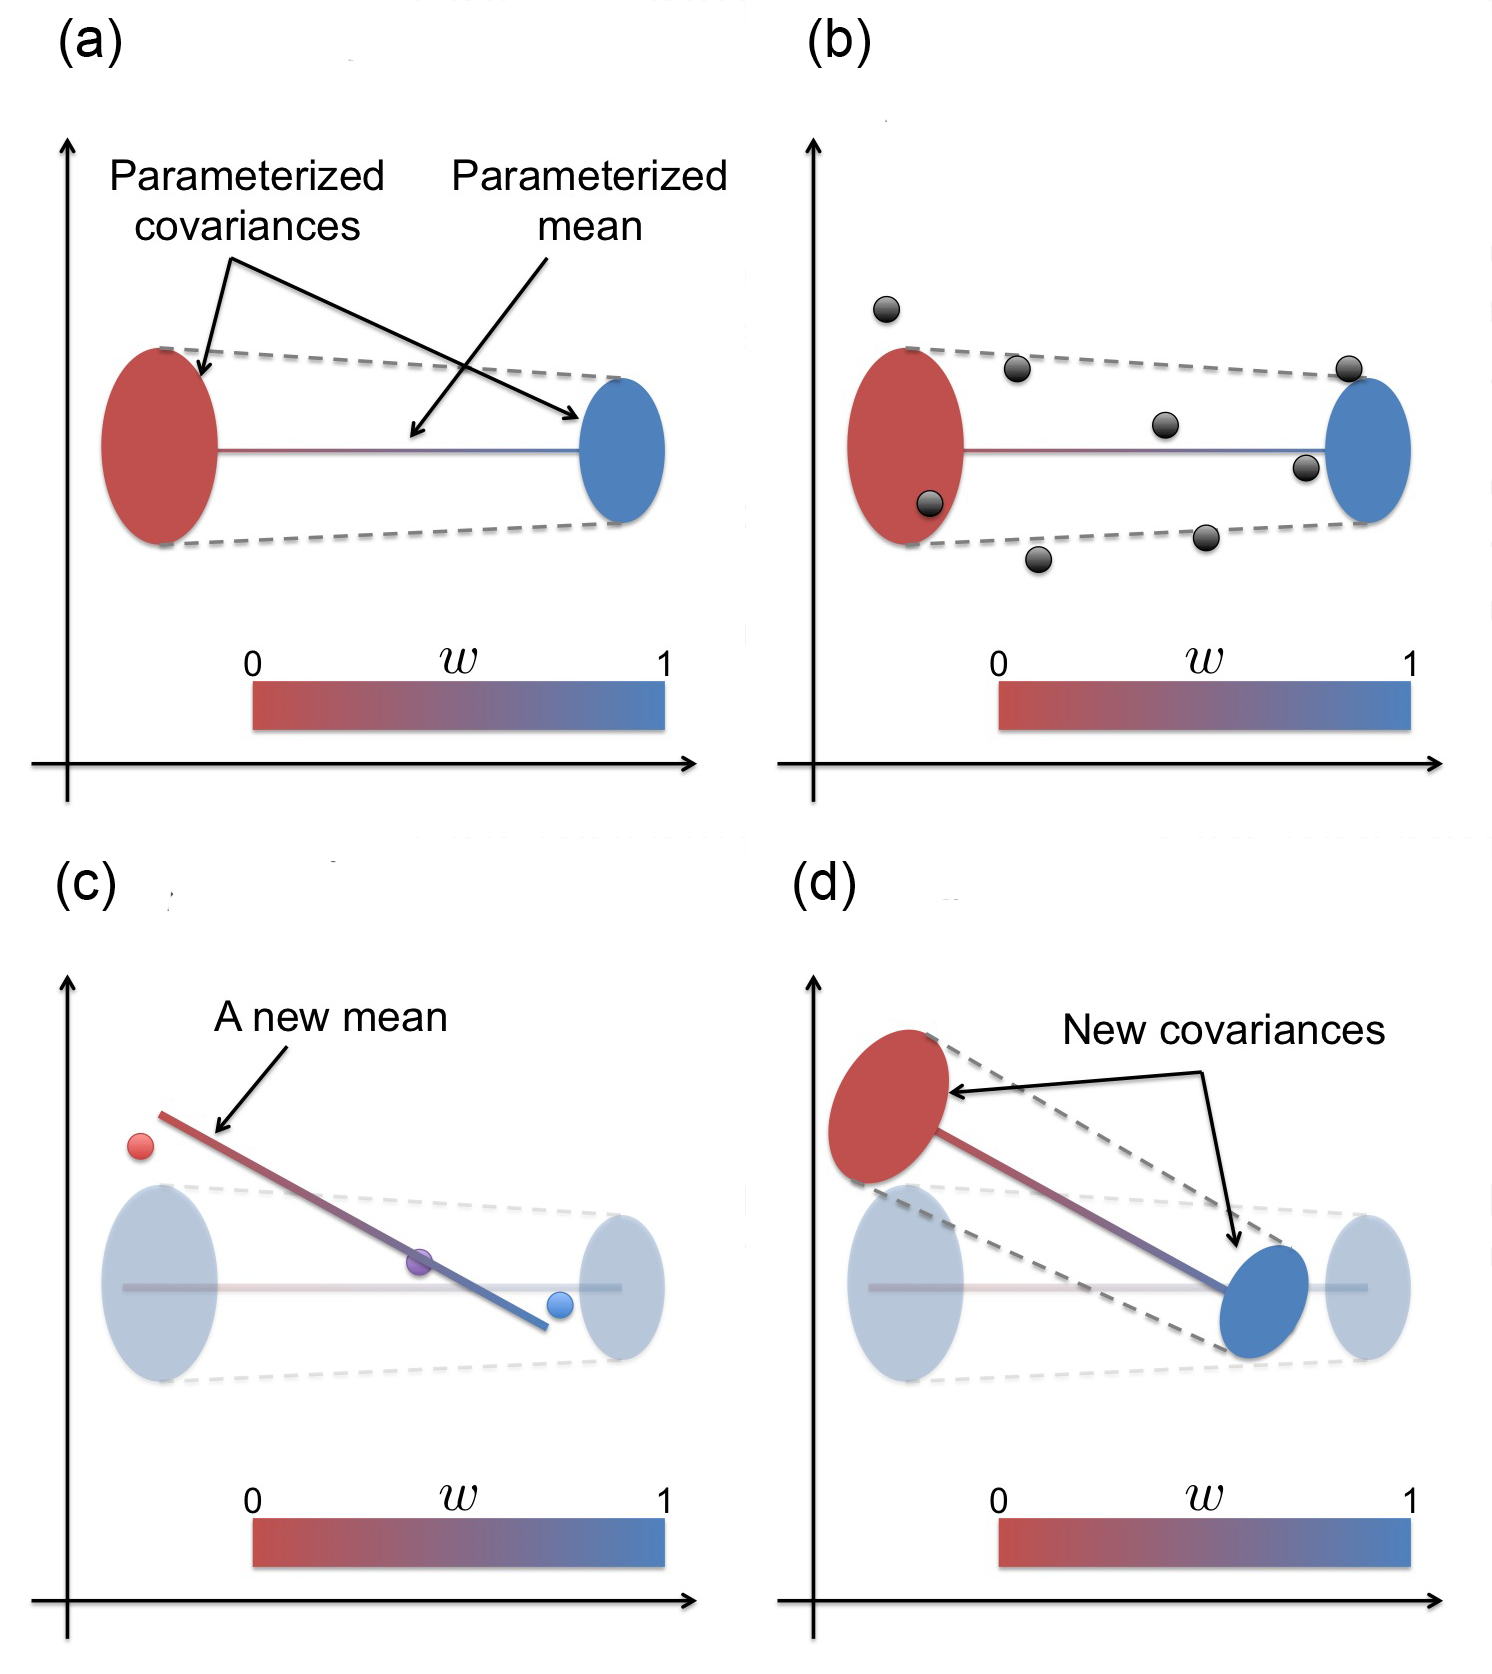
\includegraphics[width=0.75\textwidth]{images/steps}
  \caption{
    \revised{
      Steps of our algorithm for parameterized optimization problems. 
      (a) define a parameterized distribution that maps a task parameter to
      control parameters. (b) draw a set of samples from the parameterized
      distribution. (c) select the elite samples for each task and update the
      mean by applying regression. (d) update the covariances.
    }
  }
  \label{fig:optskills_steps}
\end{figure}

\revised{One iteration of our algorithms consists of three steps to update the
  parameterized distribution: drawing new samples, selecting elite samples, and
  updating the distribution (\figref{optskills_steps}).
  The following sections will describe details on each step.}

%% Three questions arise when we extend the mean from a single point to a
%% segment in the policy parameter space. How do we draw samples from the
%% current distribution, how do we evaluate and select samples, and how do we
%% update the distribution?

\subsubsection{Drawing samples}

To draw samples from the current parameterized mean
$\vc{m}_{\boldsymbol{\phi}}(w)$ and covariance matrix $\mat{C}(w)$, we
define the following probability distribution:
\begin{equation}
  \begin{aligned}
    \vc{x}_k \mytilde \frac{1}{M} \sum_{w_i \in \vc{w}}
      \Big(
      \vc{m}_{\boldsymbol{\phi}}(w_i) + \sigma \mathcal{N}(
      0, \vc{C}(w_i) ) \Big)
  \end{aligned}
  \label{eq:optskills_drawing_samples}
\end{equation} 
where $k$ is the sample index, $\sigma$ is the global step size that
controls the scale of the distribution (the details will be explained
later), and $w_i$ is one of the $M$ discretized task interpolation
parameters. This formulation is equivalent to drawing samples from a
mixture of Gaussian models with a uniform weight.

\subsubsection{Selecting samples}
We draw $\lambda$ samples from the current probability distribution
and mix the new samples with $\mu$ samples from the previous generation. From this
pool of samples, we select the best $\nu$ samples for each task $w_i$
by evaluating the task cost using \eqnref{optskills_paramcost}. We make $\nu =
\mu / M$ so that the size of elite sample set remains $\mu$ from
generation to generation. We denote each elite sample as
$\bar{\vc{x}}_i^k$, the $k^{th}$ sample for the task $w_i$.

Note that we use a set of various objective functions
(\eqnref{optskills_paramcost}) with different $w_i$ to select elite samples,
instead of a single objective function that sums up the costs over the
range of the task. We prefer specialized samples (excellent for
a particular task but mediocre on other tasks) rather than
``well-rounded'' samples (adequate for all tasks), because we need to
keep the diversity in the elite sample pool in order to evolve the
entire range of tasks. If we only keep ``well-rounded'' samples, the
sample pool will become more and more assimilated due to the single
objective function. Eventually, the mean segment will converge to a
single point instead of a curve segment.

% \updated{Please note that our selection criteria is a cost for a particular
%   task $w_i$, not a sum of costs over all tasks.
%   If we use a sum as criteria, there is one sample that is clearly better than
%   others, and it will dominate the entire population as optimization proceeded.
%   As consequence, the mean segment reconstructed from the one elite sample will
%   be a point, rather than a curve segment that we want.}

\subsubsection{Updating the model}
  After sample selection step, we can proceed to use these $\mu$ elite
  samples to update the probability model. If the new model results in
  lower objective cost, we accept the new model and move on to the
  next generation. Otherwise, we reject the new model and repeat the steps
  of drawing samples and selecting samples described above.

% \updated{One of common update mechanisms in evolutionary approaches is 
%   to generate a new candidate model and accept the candidate if its cost is
%   lower than the current model.}
% %% \karen{I thought this only applies
% %%   to (1+1) CMA-ES.} \sehoon{This is common for all elitism, $(?+?)$ selection.}
  % After sample selection step, we could proceed to use these $\mu$ elite
  % samples to fit \updated{a new candidate} mean segment

To compute a new mean segment, we apply regression on the $\mu$ elite
samples to solve for the mapping parameters $\boldsymbol{\phi}$: 
  $\vc{m}_{\boldsymbol{\phi}} (w)$. 
\begin{equation}
  \boldsymbol{\phi} = \argmin_{\boldsymbol{\phi}} \sum_{w_i \in \vc{w}} \sum_{k=1}^{\nu}\| \bar{\vc{x}}_i^{k} -
  \vc{m}_{\boldsymbol{\phi}} (w_i) \|.
  \label{eq:optskills_regression}
\end{equation}
However, using \emph{all} the selected samples tend to yield
suboptimal $\vc{m}_{\boldsymbol{\phi}}(w)$ because some samples might have
relatively high task costs (\eqnref{optskills_paramcost}). Alternatively, we could use only the
best sample for each task to fit $\vc{m}_{\boldsymbol{\phi}}(w)$, but
these best samples might not be well aligned with the assumed
function form of $\vc{m}_{\boldsymbol{\phi}}(w)$, resulting in huge error
in regression and a suboptimal mean segment.



% \updated{After the selection, the n\"aive approach to update the coefficients
%   $\boldsymbol{\phi}$ of the mean function $\vc{m}_{\boldsymbol{\phi}} (w)$ is
%   applying regression to the best samples:}
% \begin{equation}
%   \boldsymbol{\phi} = \argmin_{\boldsymbol{\phi}} \sum_{w_i \in \vc{w}} \| \bar{\vc{x}}_i^1 -
%   \vc{m}_{\boldsymbol{\phi}} (w_i) \|
%   \label{eq:optskills_regression}
% \end{equation}  
% \updated{where $\bar{\vc{x}}_i^j$ is $j$th best sample for task $w_i$.
%   However, the above regression can produce a bad mean segment if the
%   samples are not well aligned.
%   Let's consider the case that the best samples
%   $\bar{\vc{x}}_2^1,...,\bar{\vc{x}}_M^1$ are well aligned except the first sample
%   $\bar{\vc{x}}_1^1$.   
%   If the mean segment is off the samples due to the outlier $\bar{\vc{x}}_1^1$,
%   the cost can be bad and it might be better to choose another well-aligned
%   sample from the elite pool  
%   $\{\bar{\vc{x}}_1^2, \bar{\vc{x}}_1^3, ... ,\bar{\vc{x}}_1^k\}$ rather than 
%   $\bar{\vc{x}}_1^1$.}
  
We propose a new scheme to update the mean segment
$\vc{m}_{\boldsymbol{\phi}}(w)$. Instead of using \emph{all} the elite
samples or only the \emph{best} elite sample for each task, we search
for the best combination of samples such that it minimizes the task
cost and the regression error at the same
time. Our algorithm first combines samples into groups of $M$ by
randomly selecting one sample for each task $w_i$, \ie selecting one
from $\bar{\vc{x}}_i^1, \cdots, \bar{\vc{x}}_i^\nu$. Once a group
$\vc{g}$ is formed, we use the following function to evaluate the
cost of the group.
\begin{equation}
  f_{group}(\vc{g}) = \sum_{w_i \in \vc{w}} f(\bar{\vc{x}}^{g_i}_i; w_i)
  + \alpha \min_{\boldsymbol{\phi}} \sum_{w_i \in \vc{w}} \| \bar{\vc{x}}^{g_i}_i -
  \vc{m}_{\boldsymbol{\phi}} (w_i) \|
  \label{eq:optskills_group_eval}
\end{equation}  
where $g_i$ indicates the index of selected sample for task
$w_i$. $\alpha$ (=$10.0$) adjusts the weights between the task cost
and the 
%% where $\vc{g}^i$ indicates the index of selected sample for task
%% $w_i$. $\alpha$ \updated{(=$10.0$)} adjusts the weights between the task cost and the
%% >>>>>>> 0f9e6661d81053a40de7e5bb4952cc1e713277b8
regression error. Note that each evaluation of \eqnref{optskills_group_eval}
involves solving a regression for $\boldsymbol{\phi}$, but the
computational cost for regression is fairly low.

Because the number of possible groups can be potentially very large
($=\nu^M$), our algorithm only tests $100$ randomly selected groups. The function parameters
$\boldsymbol{\phi}$ that yield the best group $\vc{g}^*$ in
\eqnref{optskills_group_eval} are used to define the new mean segment:
\begin{equation}
  \boldsymbol{\phi} = \argmin_{\boldsymbol{\phi}} \sum_{w_i \in \vc{w}} \| \bar{\vc{x}}_i^{g^*_i} -
  \vc{m}_{\boldsymbol{\phi}} (w_i) \|.
  \label{eq:optskills_regression2}
\end{equation}  

The new mean segment will be compared to the
current mean by evaluating its cost (\eqnref{optskills_disccost}).
%% If the new
%% mean has a lower cost, we accept it and move on to updating the
%% covariance matrix. Otherwise, we discard the new mean and try again with
%% another set of samples redrawn from the current model.
If the new mean has a lower cost, we accept it, increase the step
size, and move on to updating the covariance matrix. Otherwise, we
discard the new mean, decrease the step size, and try again with
another set of samples redrawn from the current model.

The step size update is based on the standard 1/5-success-rule.
\begin{equation}
  \sigma = \begin{cases} 
    \sigma \cdot exp(1/3) & \text{if a new model is accepted } \\
    \sigma / exp(1/3)^{(1/4)} & \text{otherwise }
  \end{cases}
\end{equation}  

Finally, to adapt the parameterized covariance matrices, we apply the update rules used in (1+1)-CMA-ES.
For each covariance $\mat{C}(w_i)$, we call the procedure \textbf{updateCov} with
the newly accepted mean and the previous mean segments.

 % $\vc{y}(w_i)=\vc{m}_{\boldsymbol{\phi}}(w_i) -
 %  \vc{m}_{\boldsymbol{\phi}'}(w_i)$ where $\boldsymbol{\phi}'$ denotes
 %  a previous mapping coefficients.}
% Finally we control the step size using the standard 1/5-success-rule.
% \begin{equation}
%   \sigma = \begin{cases} 
%     \sigma \cdot exp(1/3) & \text{if a new model is accepted } \\
%     \sigma / exp(1/3)^{(1/4)} & \text{otherwise }
%   \end{cases}
% \end{equation}  
% \sehoon{The last sentence deleted due to the redundancy.}
%% Intuitively, this rule increases the step size if a new model is
%% accepted. Otherwise, it decreases the step size. 

%% \karen{Verify this.}
%% \updated{This rule is based on early findings in the research of evolutionary
%%   strategies \cite{Rechenberg:1994:es}. 
%% \updated{This rule tries to achieve 1/5 success rate by controlling the
%%   step size based on early findings in the research of evolutionary
%%   strategies \cite{Rechenberg:1994:es}.
%%   In short, the success rate becomes 1/2 when $\sigma$ goes to zero because
%%   very small $\sigma$ makes the objective function linear (Taylor expansion)
%%   and the linearized function has a success probability of 1/2. 
%%   On the other hand, the success rate becomes 0 when $\sigma$ is infinity
%%   because taking a large step is risky on most non-linear functions.
%%   Based on these intuition, the rule increases the step size when the current
%%   iteration was successful, and decreases on the other case.}
%% \sehoon{The reference paper said that the success rate is indeed a
%%   monotonously decreasing function in $\sigma$ on most non-linear
%%   function. Isn't this too strong?}
%% \karen{How do you define ``better''?} 

%% After the evaluation, the current sample distribution is replaced by the
%% updated distribution only if it is better than the previous one.
%% To measure the quality of the solution, we evaluate the samples along the
%% mean segment $\vc{m}_{\boldsymbol{\phi}}(w)$ (\eqnref{optskills_disccost}).
%% Although it requires $M$ additional sample evaluation,
%% it is worth because we can determine the exact quality of the current solution.
%% \karen{Don't understand this paragraph.}

